\chapter{Experiments}
The models described in section~\ref{sec:model_arch} are all tested in two test scenarios.
The offline test scenario measures the performance of the model on historical data, whereas the online scenario measures KPIs in a production setting on new data.
The reasoning behind this is that when using recommendation systems and evaluating them on historical data, the results do not necessarily reflect the real life behaviour of users.
This is because displaying recommendations changes the reality, i.e. what the user sees when using the application is different from what the user saw in the past without or with other recommendation systems.
\section{Offline}
\subsection{Experiment Setup}\label{sec:exp_setup}
In this scenario we do a temporal split and hold off future data for evaluation and train the model on historical data.
That means that the most recent sessions of each user make up the test set, while the second most recent sessions of each user make up the validation set.
Each model is evaluated on the validation set regurarly during training.
The goal of this experiment is to predict the next click of the user, given the currently active product.
After completing the training, i.e. after the validation metric does not increase anymore, the model is evaluated on the test set.
Before running the model on the MAXI dataset, some parameters were chosen based on experiments on the MIDI dataset, since due to time and resource constraints it was not possible to train all combinations of the models on the MAXI dataset.
Specifically the loss function, optimizer, batch size, learning rate, gradient clipping threshold and early stopping criterion were chosen based on the MIDI dataset, since as mentioned before it was not possible to test all these different configurations on the large dataset.
Further the one-hot encoding variants used so much time and resources, only the best performing models on the MIDI dataset were trained on the MAXI dataset.
Finally the models that used the product embedding trained much faster, therefore there were multiple versions tested for the MAXI dataset.
\par
For each model we measured two metrics of the validation set, since each of the metrics measures a different aspect of the performance of the model.
Specifically Recall@10 was measured to determine in how many cases the top 10 recommended products contained the product that was actually clicked by the user.
MRR@10 was measured to determine where the product was ranked in the top 10 predictions.
A perfect model would achieve a value of 1 in both metrics, i.e. the next clicked product is always the top prediction.
However while MRR@10 is the more informative metrics of the two, giving insight in the ranking of "good" predictions, Recall@10 is the more important one.
Achieving a Recall@10 of 1 means the next clicked item is always in the top 10 predictions, which means the user will see the recommendation, whether it is the top prediction or the fifth, which essentially is the goal of this task.
\subsection{Measurements}

\begin{table}[t]
    \centering
    \begin{tabular}{llrrr}\toprule
        \textbf{User Layer} & \textbf{Loss Function} & \textbf{RNN Units} & \textbf{MRR@10} & \textbf{Recall@10} \\ \midrule
        yes & Cross Entropy & 100 & 0.058 & 0.167 \\ 
        no & Cross Entropy & 100 & 0.069 & 0.193 \\
        yes & Top 1 & 25 & ?? & ??\todo{Get number when model is finished} \\
        yes & Top 1 & 50 & 0.081 & 0.202 \\ 
        yes & Top 1 & 100 & 0.099 & 0.226 \\ 
        yes & Top 1 & 250 & 0.073 & 0.167\todo{Verify number from most recent run} \\ 
        no & Top 1 & 25 & ?? & ??\todo{Get number when model is finished} \\ 
        no & Top 1 & 50 & 0.090 & 0.215 \\  
        no & Top 1 & 100 & 0.112 & 0.258 \\ 
        no & Top 1 & 250 & 0.121 & 0.278 \\ \bottomrule
    \end{tabular}
    \caption{Measurements on MIDI Dataset (One-Hot)}
    \label{tab:midi_dataset_measurements}
\end{table}

The measurements on the MIDI dataset are summarized in table~\ref{tab:midi_dataset_measurements}.
As mentioned above these are all measurements from the models using the one-hot encoding as input.
As can be seen the Top 1 loss introduced by the authors of~\cite{gru4rec} performs better than the cross entropy loss.
This is because the cross entropy loss essentially compares the probabilities that are predicted by the model with the "real" probability distribution, in this case with the one-hot encoding of the label.
In contrast the Top 1 loss is a strict ranking loss, only concerned with the position of the label in the predictions, which better models the task of recommendation.
Further it can be seen that the improvement of using 250 units per GRU instead of 100 is marginal, therefore larger models were not tested.
\todo{Mention results from smallest models}
Therefore the models using 250 units per GRU were chosen to be trained on the MAXI dataset in addition to the ones using the product embedding.
Finally it can be seen that the models using the user level GRU perform approximately the same, sometimes even worse than the models using only the session level GRU, the reason for this will be discussed in the next chapter.
\begin{table}[t]
    \centering
    \begin{tabular}{lrrr}\toprule
        \textbf{User Layer} & \textbf{RNN Units} & \textbf{MRR@10} & \textbf{Recall@10} \\ \midrule
        yes & 250 & 0.055 & 0.138 \\ 
        no & 250 & 0.061 & 0.146 \\ \bottomrule
    \end{tabular}
    \caption{Measurements on MAXI Dataset (One-Hot)}
    \label{tab:maxi_dataset_measurements_one_hot}
\end{table}
The measurements for the models using the one-hot on the MAXI dataset are summarized in table~\ref{tab:maxi_dataset_measurements_one_hot}.
There is nothing surprising here, again we can see that the user-level GRU apparently does not help the performance of this task.

\begin{table}[t]
    \centering
    \begin{tabular}{lrrr}\toprule
        \textbf{User Layer} & \textbf{RNN Units} & \textbf{MRR@10} & \textbf{Recall@10} \\ \midrule
        no & 25 & 0.012 & 0.025 \\ 
        no & 50 & 0.011 & 0.022 \\ 
        no & 100 & 0.012 & 0.025 \\ 
        no & 250 & diverged & diverged \\ 
        yes & 25 & 0.013 & 0.022 \\ 
        yes & 50 & 0.011 & 0.023 \\ 
        yes & 100 & 0.011 & 0.023 \\ 
        yes & 250 & diverged & diverged \\ \bottomrule
    \end{tabular}
    \caption{Measurements on MAXI Dataset (Embedding)}
    \label{tab:maxi_dataset_measurements_embedding}
\end{table}
In the table~\ref{tab:maxi_dataset_measurements_embedding} the measurements for the models using the product embedding on the MAXI dataset are summarized.
As can be quickly seen the models do not perform nearly as well as the models using the one-hot encoding.
Further the model does not improve when increasing the model size, which indicates that this is due to the product embeddings.
Also this will be a topic explored in detail in the next chapter.
\section{Online Experiment Setup}
\subsection{Experiment Setup}
In this scenario we train the models on all the available data and evaluate the performance on live data generated by users that use the web application.
For this we chose the best performing configuration for each variant (c.f.~\ref{tab:model_archs}) from the offline experiments.
Using these four models an A/B/C/D/E test was setup.
An A/B/n test is often used when testing features for online services.
Such a test consists of choosing different versions of the same element or feature and then partition the traffic into groups, where each group is assigned to one version of the element.
One of the versions should always serve as a control group, receiving the original version of the element.
The user to group assignment is done at random to get evenly distributed groups.
This group assigment is also persistent across different sessions.
After such a test is setup, the test is run for some time while measuring KPIs per group.
Then after ending the test the best performing version can be chosen based on the KPIs measured during the test.
\par
The element that was tested in this work is the first slot for recommendations on the product detail page, the page that receives the most traffic.
The slot is illustrated in figure~\ref{fig:ab_test_slot}.
\begin{figure}[t]
	\centering
	\captionsetup{width=0.8\textwidth}
    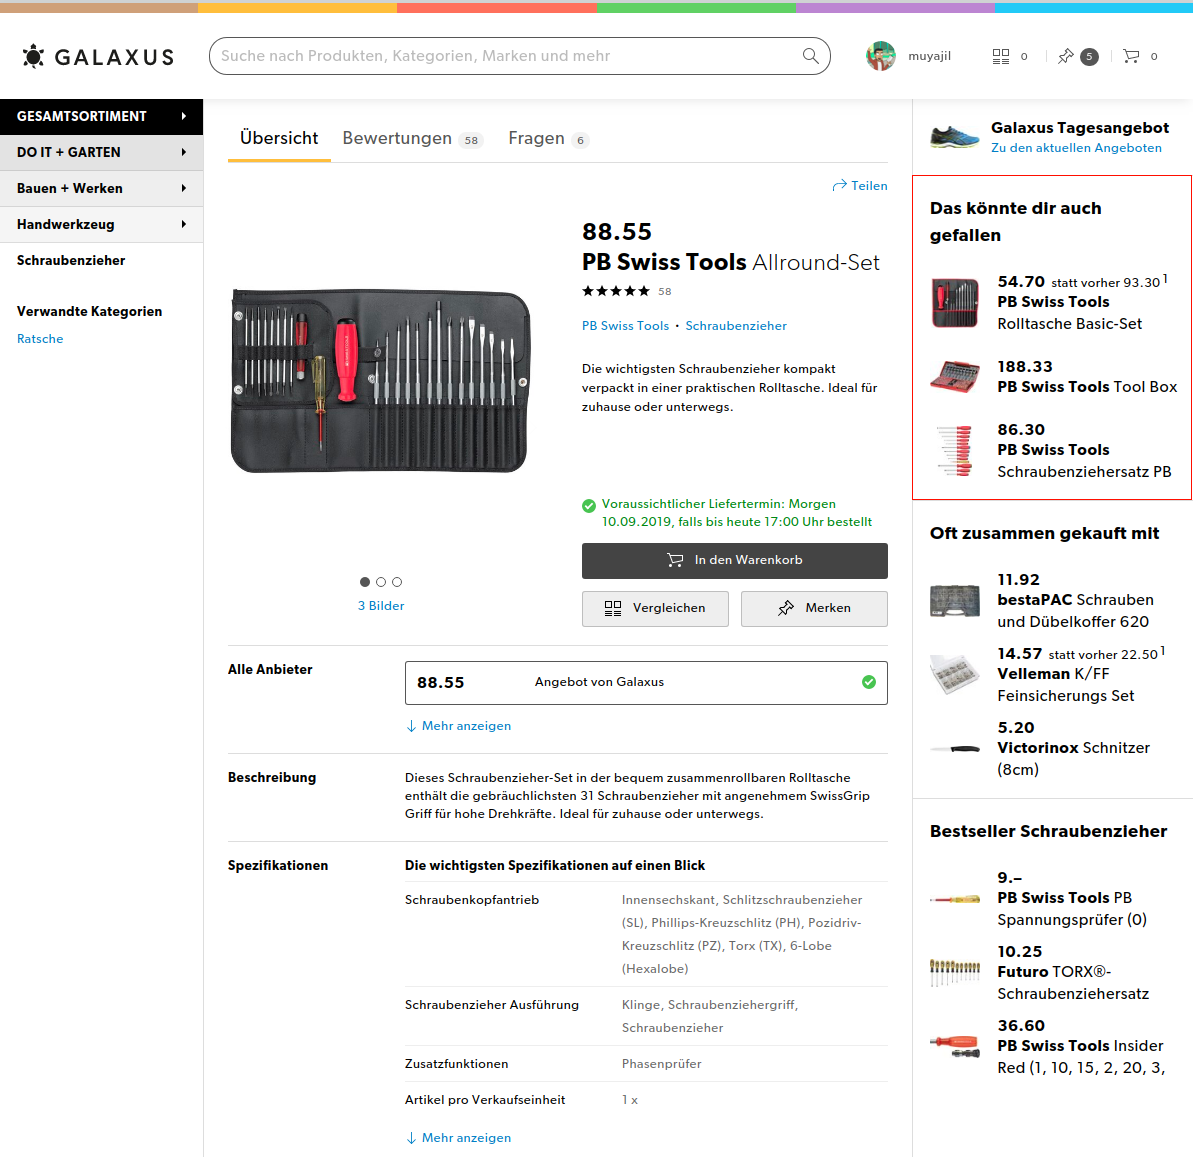
\includegraphics[width=\textwidth]{ab_test_slot.png}
    \caption{Recommendation slot on the product detail page}
    \label{fig:ab_test_slot}
\end{figure}
As a control version a black-box recommendation system provided by Google called Recommendations AI~\footnote{\url{https://cloud.google.com/recommendations/}} was chosen.
In the normal mode the chosen recommendation slot still has multiple recommendation engines which can be chosen according to a framework, however Recommendations AI is the best performing one.
Other than the logic chooses the products to display nothing was changed, i.e. the title and design remained identical.
The test was run for 14 days to reflect one whole business cycle.
\par
Something important to note at this stage is the postprocessing of recommendations coming either from the tested model or Recommendations AI.
There are some constraints that are applied on the recommended product, such as filtering products that are inappropriate (e.g. alcoholic beverages, erotic articles etc.) and products that are not available for sale anymore (e.g. discontinued products, not on stock).
This post processing is applied on all recommendation engines, therefore still providing a leveled playing field.
However this is one of the reasons why production testing makes sense for recommendation systems, since this can never be reproduced in an offline setting, since some of these factors change over time.
\subsection{Measurements}
In table~\ref{tab:online_measurements} we can see the measurements for the different variants of the model in the online setting, as well as the same metric for different models that have been displayed in the same slot as the one we tested in.
We focus on the Click-Through rate in this experiment, since as mentioned before the conversion rate is difficult to compute, and due to time constraints we could not wait 14 days after the test was finished to get a good estimation of this metric.
The test was executed on approximately 1.3 Million sessions, each of the variants, as well as Recommendations AI received 20\% of the total traffic coming to the product detail page.
The metrics for each of the recommendation engines is averaged over all the sessions.
\begin{table}[ht]
    \centering
    \begin{tabular}{lr}\toprule
        \textbf{Model Name} & \textbf{CTR} \\ \midrule
        OnlySessionOneHot & 2.1\% \\
        OnlySessionEmbedding & 0.85\% \\
        WithUserOneHot & 2\% \\
        WithUserEmbedding & 0.9\% \\
        Recommendations AI & 5.55\% \\
        OftenBoughtTogether & 0.91\%* \\
        SimilarProducts & 1.19\%* \\ \bottomrule
    \end{tabular}
    \caption{Measurements on Live Data \\ (* Values are not based on the same test, but instead on more than 2 years of data.)}
    \label{tab:online_measurements}
\end{table}
\par
OftenBoughtTogether is a simple heuristic counting which products are bought with which other products\todo{other formulation}.
It is very similar to the one described in section~\ref{sec:often_bought_together}.
Similar Products is a recommendation engine also using the product embeddings produced by Meta-Prod2Vec.
This engine will recommend the items that are closest to the currently active item in the embedding space.
\par
As can be seen in table~\ref{tab:online_measurements} nothing comes close to achieving the same result as Recommendations AI.
This is a proprietary system which is acessed directly via an API, however the data that is ingested by this system is very diverse.
The system does not only consider the currently viewed item and the active user, but also takes into account trends, recent sales, product information and more.
However when compared to more classical approaches the session-based approach performs much better, at least when using the one-hot encoding, since also in this setting we can see that the models using the product embedding perform much worse.